% Chapter Template

\chapter{Test setup and results} % Main chapter title

\label{Chapter5} % Change X to a consecutive number; for referencing this chapter elsewhere, use \ref{ChapterX}

\lhead{Chapter 5. \emph{Test setup and results}} % Change X to a consecutive number; this is for the header on each page - perhaps a shortened title

After discussing how crawl.js works we want to introduce our setup environment and discuss some results. We decided to test crawl.js in a closed environment. Crawling the public internet requires a good supervision and the required work to do that is simply out of scope for this thesis. All experiments were done on the opennebula cluster hosted at the university of neuchatel.

During our experiments we want to verify the following basic properties of crawl.js:
\begin{itemize}
\item All pages are found (starting with a single seed URL)
\item The crawl stops
\item Adding more workers reduces the crawl time
\end{itemize}

Furthermore we want to verify the \emph{closeness}~\ref{closeness} aspect of crawl.js. Crawl.js is configurable in such a way that sites that are \emph{close} (in terms of latency) to a worker are assigned to them. In order to do that we will add virtual latency to some of the sites and compare two different mapper~\emph{mapper} implementations:
\begin{itemize}
\item Simple - the whole URL is hashed. Therefore the site to worker assignment is random.
\item 2-level - the host part of the URL identifies the group of workers. (a group that is \emph{close}). The remaining part of the URL determines the worker inside the group.
\end{itemize}

\section{Test setup}
To do our experiments we had to setup the following types of VM in the cluster:
\begin{itemize}
\item www - static wikipedia snapshots.
\item redis - remote queues.
\item workers - crawls pages from \emph{www} and updates remote queues in \emph{redis}.
\end{itemize}

To setup and manage (workers) the VMs efficiently we wrote some basic bash scripts. They allow us to deploy different worker configurations easily and perform basic operations on the workers such as start and stop. Having those scripts saved us a lot of time throughout the different experiments we ran. You find them in our crawl.js git repository. In Figure~\ref{test_setup} is an overview of all the VMs used during the experiments.

\begin{figure}[h]
\centering
  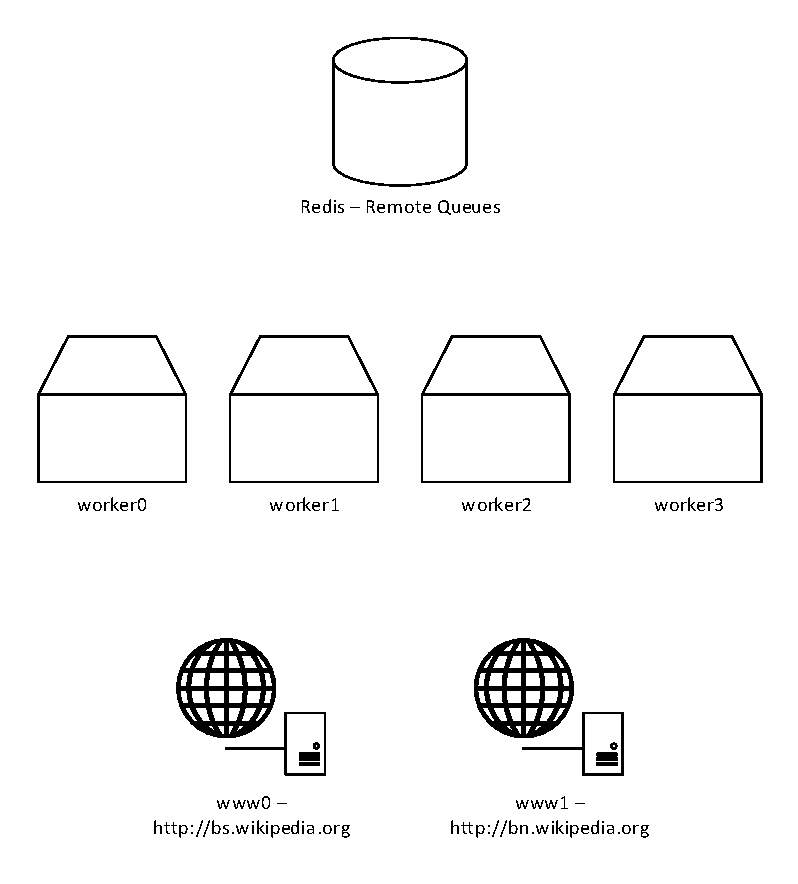
\includegraphics[width=1\textwidth]{Figures/test_setup.pdf}
\caption{Crawl.js - Test setup overview}
\label{test_setup}
\end{figure}

\subsection{www - wikipedia snapshots}
In order to have realistic sites to crawl we decided to setup wikipedia html dumps. Unfortunately their dumper stopped back in 2008 and therefore the snapshots are pretty old. But for our usecase it is good enough. Almost. Back then, the different wikipedia langages were located in different subdirectories. All on the same server. But we need links pointing to different servers to test the discussed \emph{closeness} aspect of crawl.js. Therefore we wrote an xsl transformation script to change all language links from www.wikipedia.org/de/index.html to de.wikipedia.org/index.html. You find those scripts in our repository.


Additionally we encountered a serious performance problem during our first tests. The random read performance in our VM was about 200 IOPS (tested with fio). Therefore the webserver (nginx) could not deliver pages fast enough and represented the bottleneck in our setup. In order to circumvent this unwanted side effect we put our html dumps on a ramfs.

\begin{itemize}
  \item CPU: 1, VCPU: 1
  \item RAM: 2048M
\end{itemize}

\subsection{redis - Remote queues}
This setup was pretty simple. Just a single redis server instance running. Because all the URLs have to fit in memory, setting up a redis cluster to share the keyspace on different servers is inevitable as soon the number of URLs becomes too big. In our simple/small setup this was not needed. During our experiments we encountered 217'690 URLs which represents 82M of data inside the redis server (redis info command).

\begin{itemize}
  \item CPU: 1, VCPU: 1
  \item RAM: 3072M
\end{itemize}

\subsection{worker - Crawl.js worker instance}
The worker VM hosts our developed crawler (crawl.js instance). Setting it up was staight forward. First we thougt that we could host more than one crawler instance (using multiple cpus) but we achieved better results whith one crawler per worker. This 1:1 worker to crawler relation made the managment easier too. Setup and managment scripts are available in our repository.

\begin{itemize}
  \item CPU: 1, VCPU: 1
  \item RAM: 1024M
\end{itemize}

\section{Experiment 1 (basic properties, scaling)}
This experiment was about verifying the basic properties of crawl.js as discussed in section~\ref{Chapter5}.
Configuration:
Mapper: simple
#workers: 1 - 4

Figure~\ref{exp_001} shows our first results.

\begin{tikzpicture} \begin{axis}[xbar,enlargelimits=0.15]
\addplot
[draw=blue,pattern=horizontal lines light blue] coordinates
    {(10,5) (15,10) (5,15) (24,20) (30,25)};
\addplot
[draw=black,pattern=horizontal lines dark blue]
coordinates
    {(3,5) (5,10) (15,15) (20,20) (35,25)};
\end{axis}
\end{tikzpicture}
